\section{Result Evaluation}
\label{sec:result}
In this section, we will analyze the performance of the dynamic hybrid prefetcher. In Fig. \ref{fig:final_acc_cov}, the accuracy and coverage data is displayed. The accuracy performance is similar to the one from \emph{Brute Force Search}, while much less than \emph{ISB}'s and \emph{Static Analysis}'s. The coverage performance is better than the one from \emph{Brute Force Search}, similar to \emph{ISB}'s and \emph{Static Analysis}'s. These are fairly good since before the first 1024 accesses of \emph{ISB} or first 512 accesses of \emph{BO}, the prefetcher acts as a naive hybrid prefetcher.

\begin{figure}[ht!]
   \centering
   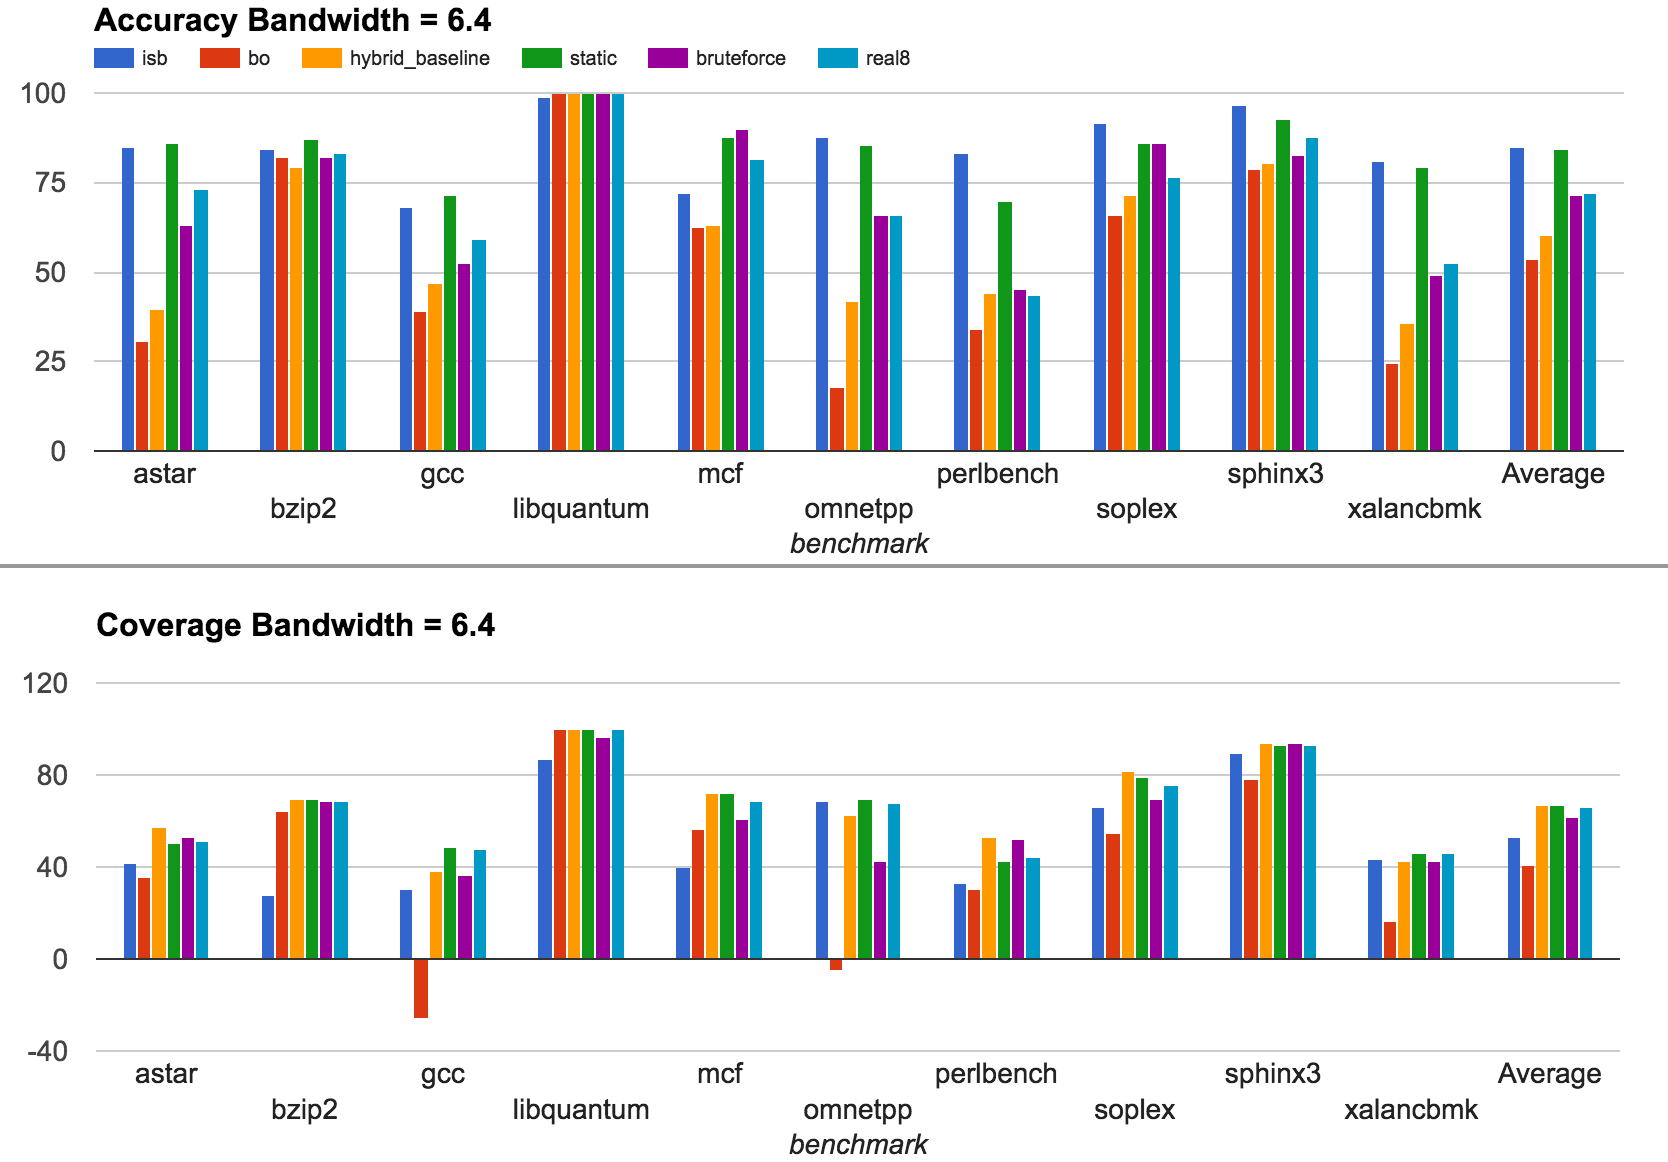
\includegraphics[width=1.0\textwidth]{images/final_acc_cov.png}
   \caption{Accuracy and coverage performance of dynamic hybrid prefetcher}
   \label{fig:final_acc_cov}
\end{figure}

In terms of speedup, as shown in Fig. \ref{fig:final_speedup}, the dynamic hybrid prefetcher is 6\% better than baseline but 6\% away from the \emph{Brute Force Search} headroom. Since we were doing project on Akanksha's shoulder, 6\% is a pretty good result. However, \emph{DHP}'s accuracy and coverage is higher. There are several reasons we think may account for thisi fact.
\begin{itemize}
  \item The training overhead. The decision only start after certain number accesses are made.
  \item The heuristic drawn from \emph{Static Analysis} focuses on improving accuracy and coverage instead of speedup.
  \item Memory pressure are ignored. Some prefetches should have been issued are not issued, vice versa.
  \item \emph{DHP} cannot react to phase change fast enough.
  \item The heuristic itself has some inperfection after applied to \emph{DHP}.
\end{itemize}

\begin{figure}[ht!]
   \centering
   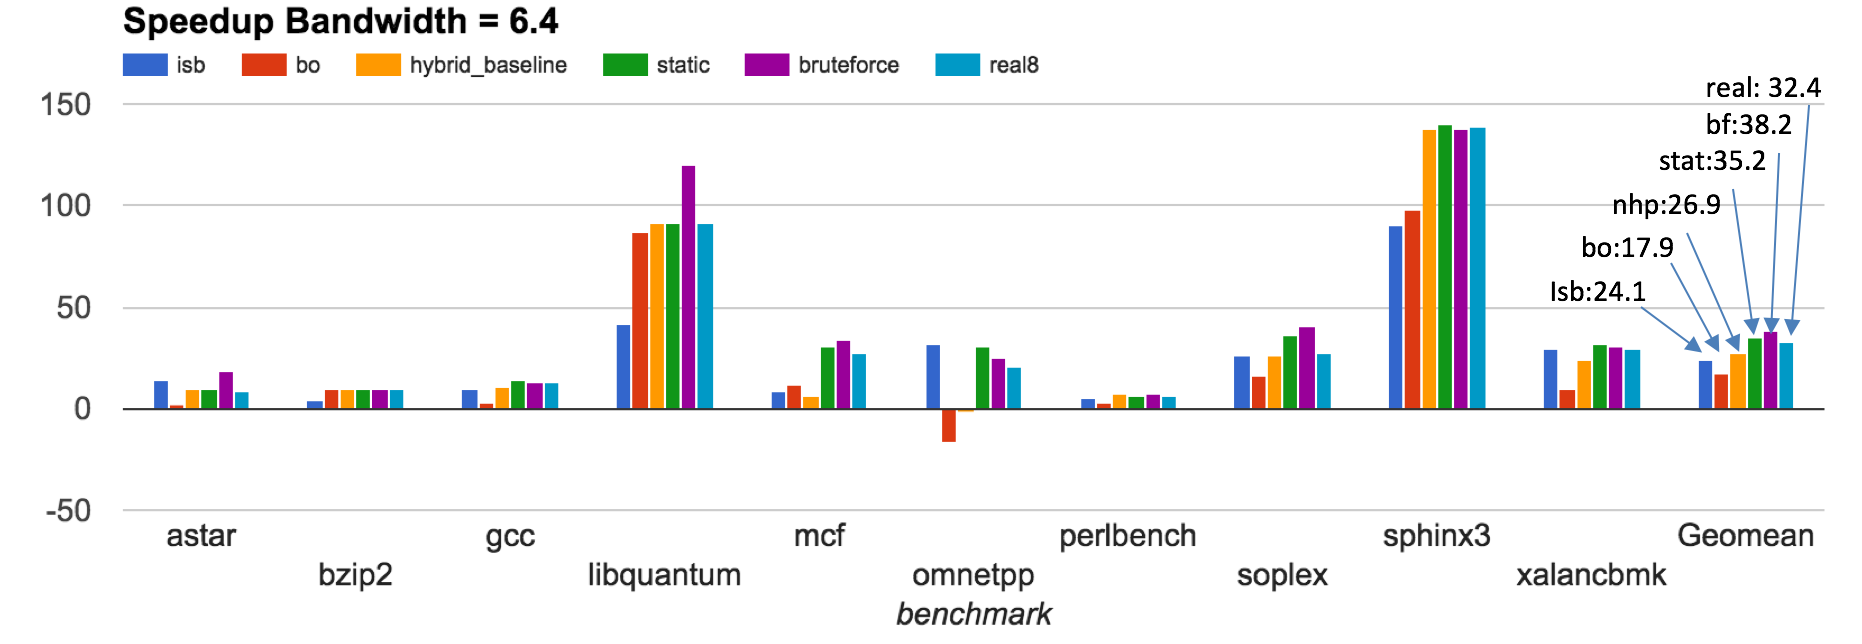
\includegraphics[width=1.0\textwidth]{images/final_speedup.png}
   \caption{Speedup performance of dynamic hybrid prefetcher}
   \label{fig:final_speedup}
\end{figure}

\subsubsection*{}
As a test, we accually tried to monitor memory usage in real time. We measured the number of accesses in one period to represent the memory bus pressure. When the usage is high, then just prefetch \emph{ISB}'s decision if BOTH is met. On the other hand, increase the number of prefetchings when memory usage is low. Fig. \ref{fig:final_speedup_mem} shows our result. Unfortunately, this turns out to be a difficult problem. The naive measurement we've done seems problematic when guiding the \emph{DHP}'s decision. Maybe the timeliness of this measurement make \emph{DHP} make many wrong decisions. However, this path do have potential to improve \emph{DHP}'s performance.

\begin{figure}[ht!]
   \centering
   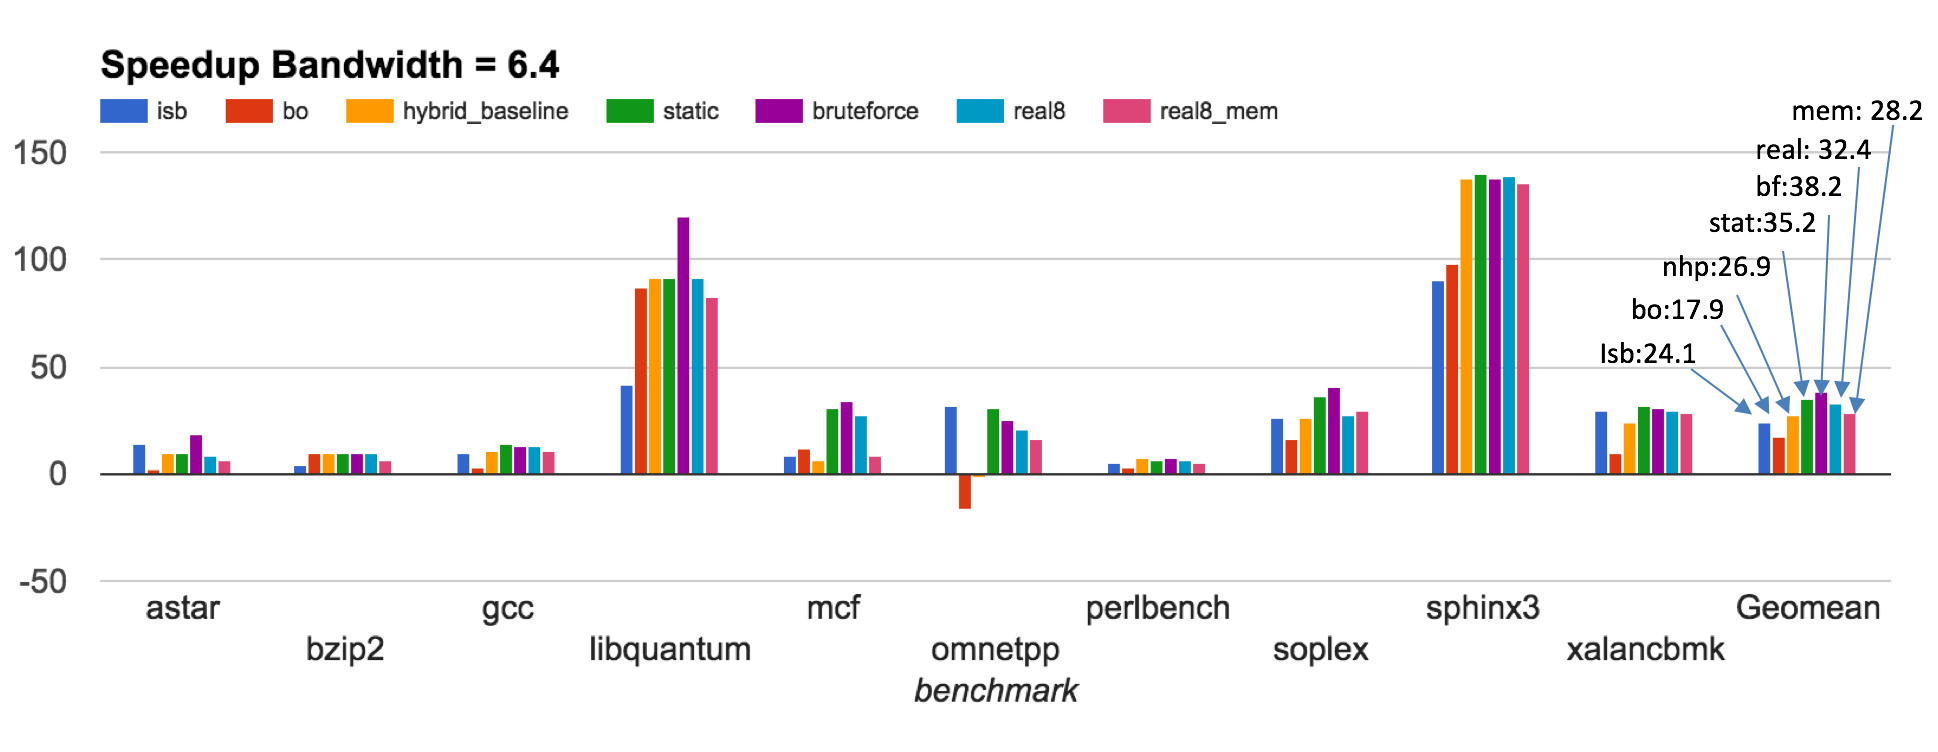
\includegraphics[width=1.0\textwidth]{images/final_speedup_mem.png}
   \caption{Speedup performance of dynamic hybrid prefetcher when consider memory pressure}
   \label{fig:final_speedup_mem}
\end{figure}
